% !TEX root = ../pdf/stat205.tex
% [There are multiple stat205.tex files, but the one in ../pdf is the usual one]



%%%%%%%%%%%%%%%%%%%%%%%%%%%%%%%%%%%%%%%%%%%%%%%
\chapter{Estimation}


\begin{verse}{\it
``When there are but two players, your theory which proceeds by combinations is very just. \\
But when there are three, I believe I have a proof that it is unjust that you should proceed in any other manner than the one I have.''\vspace*{6pt}} \\
\hspace*{2cm} -- Pascal's letter to Fermat\FOOTNOTE{from \url{https://www.york.ac.uk/depts/maths/histstat/pascal.pdf}}
\end{verse}
\vspace*{12pt}


\section{Introduction}

In previous chapters, we worked with problems where the sample space was fully known.
For instance, in Examples \autoref{exmp:coin_toss} and \autoref{exmp:heads_observe}, we knew that the coin was fair and that it could only land on heads or tails.
In Example \autoref{exmp:three_balls_urn}, we had complete information about the number of balls in the urn and their respective colors.
Example \autoref{exmp:eye_color} provided us with the exact frequency distribution of eye colors among town residents.
In Example \autoref{exmp:women_heights}, we were given that women's heights in the city followed a normal distribution, and so on.

In this chapter, we will work with statistical problems.
Unlike in previous examples, we do not know the bigger picture in these cases.
However, we have some information that comes from this bigger picture.
For example, we can draw balls from an urn without being able to see what's inside.
Or we might randomly select some women from Example \autoref{exmp:women_heights}, measure their heights, and use these observations to learn about their height distribution.

As another example, consider tossing a coin 500 times when we don't know whether it's fair or biased.
Suppose we get 243 heads.
We might then estimate a parameter such as \( p \), the probability of heads, as \( \frac{243}{500} = 0.486 \) using this frequentist approach.
However, this approach involves uncertainty.
For instance, another experiment might yield 225 heads, or someone might use a different method than the frequentist approach to estimate \( p \).
Therefore, the estimate of \( p \) cannot be determined with perfect accuracy.
In statistics, we study methods and principles to find the best possible estimates for unknown parameters like \( p \).

\keyterm{Inferential statistics} is the branch of statistics concerned with drawing conclusions and making inferences from data analysis.
In this section, we focus on estimation methods for determining optimal approximations of unknown parameters,
while the next section covers hypothesis testing.

\section{Estimation of Parameters}

Consider a discrete or continuous random variable  \( X \).
For example, \( X \) could be the number of children in households in a city (a discrete random variable) or the height of citizens in the city (a continuous random variable).
In the first case, \( X \) is defined for households, and in the second, it is defined for individuals.

Alternatively, \( X \) can represent the outcome of a random experiment.
For instance, when tossing a coin, the result of interest could be the outcome of the coin toss (a discrete random variable) or the time it takes for the coin to land after leaving the hand (a continuous random variable).

The studied instances (households, individuals, trials of a random experiment, etc.) are called the \keyterm{population}.
The population size is typically denoted by \( N \).

Suppose we know the PDF of \( X \), but it depends on one or more unknown parameters.
For instance, in a Bernoulli trial, \( X \) follows a Bernoulli distribution with unknown parameter \( p \).
While it would be ideal to record the variable of interest for every member of the population to determine \( p \), this is often impractical.
The population may be too large, making such calculations time-consuming, impossible, or expensive.
Instead, we gather information from a smaller subset of the population, called a \keyterm{sample}.
The sample size is typically denoted by \( n \).

\subsection{Statistic}

Suppose \( X \) follows a distribution \( f(x; \theta) \), where \( \theta \in A \) is an unknown \keyterm{parameter}.
The set \( A \) of all possible values for \( \theta \) is called the \keyterm{parameter space}.
For example, if \( X \) is a Bernoulli variable with success probability \( \theta \),
then \( 0 \leq \theta \leq 1 \), and so \( A = [0, 1] \) is the parameter space.


The parameter may also be a \( k \)-dimensional vector, denoted \( \bm{\theta} = (\theta_1, \theta_2, \ldots, \theta_k) \).
For instance in a normal distribution, \( \theta = (\mu, \sigma) \) is a two-dimensional parameter.

A \keyterm{statistic} is a function \( U = g(X_1, X_2, \ldots, X_n) \) of a random sample \( X_1, X_2, \ldots, X_n \) that does not depend on unknown parameters.
By definition, a statistic is itself a random variable (since it is a function of random variables).
The distribution of \( U \) may or may not depend on the parameters.
For example, if \( X_1, X_2, \ldots, X_n \) is a random sample from \( N(\mu, 1) \),
then the sample mean \( U = \bar{X} = \frac{X_1 + X_2 + \ldots + X_n}{n} \) follows a normal distribution \( N(\mu, \frac{1}{n}) \) by the Central Limit Theorem (CLT).
Here, the distribution of \( U \) depends on the mean parameter \( \mu \).

\subsection{Estimator and Estimate}

If we observe the values \( x_1, x_2, \ldots, x_n \) for the random sample \( X_1, X_2, \ldots, X_n \)
and compute the statistic \( u = g(x_1, x_2, \ldots, x_n) \),
we can use \( u \) as an estimation of the parameter \( \theta \).
In this context, \( U = g(X_1, X_2, \ldots, X_n) \) is called an \keyterm{estimator} of \( \theta \),
while the computed value \( u \) is called an \keyterm{estimate} of \( \theta \).

Note that an estimator is itself a statistic and is therefore a random variable.
Thus, both estimators and statistics are denoted by capital letters.
In contrast, estimates (observed values) are denoted by lowercase letters.
Also, while every estimator for \( \theta \) is a statistic,
not every statistic serves as an estimator for \( \theta \).

\begin{exmp}
    Suppose \( X \) represents a country's annual GDP growth, where \( X \sim N(\mu, 0.2) \).
    We want to estimate \( \mu \) based on this random sample:
    \[ 1.1, 1.6, 2.4, 3.2 \]
    Since \( \mu \) is the mean of \( X \), observing multiple realizations of \( X \) should allow us to estimate \( \mu \).
    For instance, the sample mean of these observations seems like a proper estimate for \( \mu \):
    \begin{gather*}
        u = \bar{x} = \frac{1.1 + 1.6 + 2.4 + 3.2}{4} = 2.075
    \end{gather*}
    The corresponding estimator is:
    \begin{gather*}
        U = \bar{X} = \frac{X_1 + X_2 + X_3 + X_4}{4}
    \end{gather*}
\end{exmp}
\begin{exmp}
    Consider a population of \( N = 1423 \) accident-involved individuals, where \( p \) denotes the proportion who drink excessively.
    The proportion of them in a random sample \( \hat{p} \) may be used to estimate \( p \).
\end{exmp}
In the previous two examples, \( \bar{X} \) and \( \hat{p} \) are called \keyterm{point estimators}.
Deriving point estimators is one way of estimating population parameters.
Ideal point estimators possess some characteristics.
For instance, we want low variance, meaning the point estimates don't vary widely across different samples.

While various methods exist for deriving point estimators, we focus instead on confidence intervals – interval estimates that capture the parameter of interest with a specified level of confidence.

\section{Confidence Intervals}

To better understand confidence intervals, let's start with an example:

\begin{exmp}
    Let \( X_1, X_2, \ldots, X_{100} \) be a random sample from \( X \sim N(\mu, 9) \).
    What is the probability that the unknown parameter \( \mu \) lies in the interval \( (\bar{X} - 0.3, \bar{X} + 0.3) \)?
\end{exmp}
\begin{solution}
    We know from the Central Limit Theorem that \( \bar{X} \sim N(\mu, \frac{\sigma^2}{n}) = N(\mu, 0.09) \),
    and therefore after standardization, \( \frac{\bar{X} - \mu}{\frac{\sigma}{\sqrt{n}}} = \frac{\bar{X} - \mu}{0.3} \sim N(0, 1) \). Thus:
    \begin{align*}
        P(\bar{X} - 0.3 < \mu < \bar{X} + 0.3) &= P(-1 < \frac{\bar{X} - \mu}{0.3} < 1)\\
        &= P(-1 < Z < 1)
    \end{align*}
    which equals:
    \begin{lstlisting}[language=R]
> pnorm(1) - pnorm(-1)
[1] 0.6826895
    \end{lstlisting}
\end{solution}
Note that we call the interval \( (\bar{X} - 0.3, \bar{X} + 0.3) \) in the previous example a \emph{random interval} since it has two random variables as its endpoints.
This random interval contains the parameter \( \mu \) with approximately 68\% probability.
From a frequentist perspective, this implies that if we were to construct 100 such intervals from different random samples, we would expect about 68 of them to contain the true parameter \( \mu \).
For example, one such interval might be \( (1.6, 2.2) \) when the sample mean is \( \bar{x} = 1.9 \).
We call such an interval a 68\% confidence interval.
But note that this does not mean \( (1.6, 2.2) \) contains the parameter \( \mu \) with 68\% probability!
\( (1.6, 2.2) \) is an observed interval, and it already either contains \( \mu \) or not.

Let \( U \) be a point estimator for \( \theta \) based on a random sample from \( f(x; \theta) \).
Consider the random interval \( (g_1(U), g_2(U)) \), where \( g_1(U) \) and \( g_2(U) \) are functions of \( U \).
If
\begin{gather*}
    P(g_1(U) < \theta < g_2(U)) = 1 - \alpha
\end{gather*}
for some constant \( 0 \leq \alpha \leq 1 \) (independent of \( \theta \)),
then this interval is called a \keyterm{\( 100(1 - \alpha)\% \) confidence interval} (or a confidence interval with confidence level \( 1 - \alpha \)) for the parameter \( \theta \).

As we will later see, the structure of our confidence intervals is
\begin{gather*}
    (\text{point estimator} - \text{margin of error}, \text{point estimator} + \text{margin of error})
\end{gather*}
As the confidence level \( 1 - \alpha \) approaches 1 and the average margin of error \( E(\text{margin of error}) \) decreases,
we gain both higher confidence that the interval contains the true parameter value and a more precise (narrower) interval estimate (see Example \autoref{exmp:lifespan_ci}).

\subsection{Confidence Interval for Mean Parameter}

We consider two cases:
\begin{enumerate}
    \item \( \sigma^2 \) is known:
    
    \( \bar{X} = \frac{X_1 + X_2 + \ldots + X_n}{n} \) follows a normal distribution \( N(\mu, \frac{\sigma^2}{n}) \) by the Central Limit Theorem (CLT).
    Thus, \( Z = \frac{\bar{X} - \mu}{\frac{\sigma}{\sqrt{n}}} \sim N(0, 1) \).
    \begin{figure}[t]
    \begin{center}
    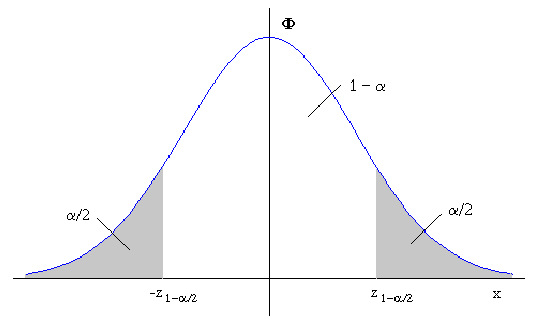
\epsfig{file=../img/The-1-a-quantiles-of-the-normal-distribution.png,clip=true,width=15cm}
    \end{center}
    \caption{Image is from \href{https://www.researchgate.net/figure/The-1-a-quantiles-of-the-normal-distribution_fig2_273257392}{ResearchGate}}
    \label{fig:the-1-a-quantiles-of-the-normal-distribution}
    %\HR
    \end{figure}
    As illustrated in \autoref{fig:the-1-a-quantiles-of-the-normal-distribution}, we have:
    \begin{gather*}
        P(-z_{1 - \frac{\alpha}{2}} < \frac{\bar{X} - \mu}{\frac{\sigma}{\sqrt{n}}} < z_{1 - \frac{\alpha}{2}}) = 1 - \alpha
    \end{gather*}
    where \( z_\gamma \) is defined such that \( P(Z \leq z_\gamma) = \gamma \) for \( \gamma \in [0, 1] \).
    So for example, \( z_{1 - \frac{\alpha}{2}} \) is the point on the standard normal distribution where the accumulated probability to its left is \( 1 - \frac{\alpha}{2} \).
    Note that as shown in \autoref{fig:the-1-a-quantiles-of-the-normal-distribution}, by symmetry we have  \( z_{\frac{\alpha}{2}} = -z_{1 - \frac{\alpha}{2}} \).
    By solving the two inequalities in the probability above, we obtain the confidence interval below for \( \mu \):
    \begin{gather*}
        (\bar{X} - z_{1 - \frac{\alpha}{2}}\frac{\sigma}{\sqrt{n}}, \bar{X} + z_{1 - \frac{\alpha}{2}}\frac{\sigma}{\sqrt{n}})
    \end{gather*}
    \item \( \sigma^2 \) is unknown:
    
    In practice, we almost never know the value of the variance \( \sigma^2 \), since by definition:
    \begin{gather*}
        \sigma^2 = \frac{\sum_{i = 1}^{N}(x_i - \mu)^2}{N}
    \end{gather*}
    while \( \mu \) is unknown, and our goal is to estimate it!

    Hence, we use the sample variance \( S^2 \) instead of \( \sigma^2 \), which is defined as:
    \begin{gather*}
        S^2 = \frac{\sum_{i = 1}^{N}(x_i - \bar{x})^2}{n - 1}
    \end{gather*}
    It can be proved that \( \frac{\bar{X} - \mu}{\frac{S}{\sqrt{n}}} \) follows a \keyterm{(Student's) t-distribution} with \( n - 1 \) \keyterm{degrees of freedom (df)},
    denoted \( T_{n - 1} = \frac{\bar{X} - \mu}{\frac{S}{\sqrt{n}}} \sim t_{n - 1} \).

    The t-distribution resembles the normal distribution in several key aspects: it is symmetric, unimodal, and bell-shaped.
    Its shape is determined by the degrees of freedom (df) parameter which usually takes integer values, with larger df values making it increasingly similar to the standard normal distribution.
    \autoref{fig:t_distribution} shows the t-distributions with degrees of freedom (df) 1, 5, and 30, along with the standard normal distribution for comparison.
    As evident from the plot, the t-distribution with \( df \geq 30 \) closely aligns with the normal distribution, demonstrating their convergence at higher degrees of freedom.
    \begin{figure}[t]
    \begin{center}
    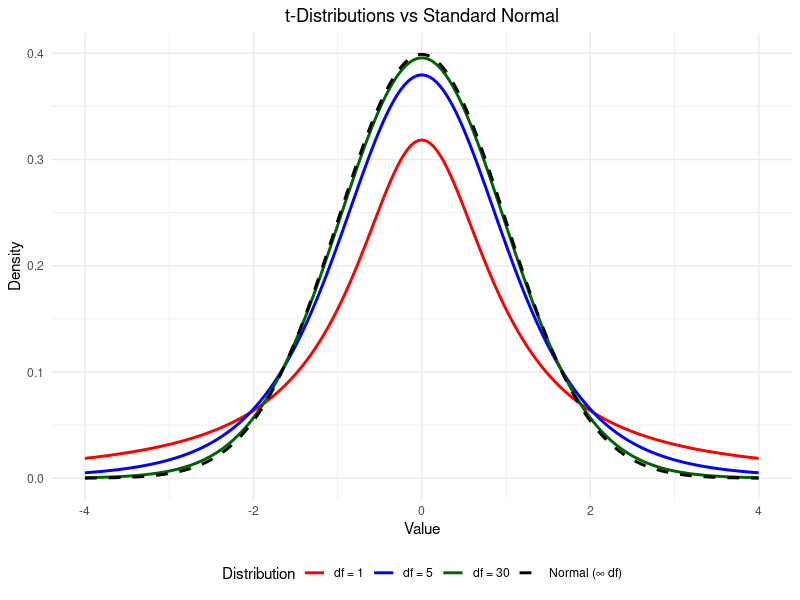
\epsfig{file=../img/t_distribution_plot.png,clip=true,width=15cm}
    \end{center}
    \caption{Comparison of t-distributions with degrees of freedom (df) = 1, 5, and 30 against the standard normal distribution (black dashed line). The t-distribution approaches normal distribution as df increases, with df = 30 (dark green) nearly overlapping the standard normal distribution.}
    \label{fig:t_distribution}
    %\HR
    \end{figure}

    Due to its similar bell-shaped symmetry to the normal distribution, the same reasoning as the previous case applies, yielding the confidence interval:
    \begin{gather*}
        (\bar{X} - t_{1 - \frac{\alpha}{2}, n - 1}\frac{S}{\sqrt{n}}, \bar{X} + t_{1 - \frac{\alpha}{2}, n - 1}\frac{S}{\sqrt{n}})
    \end{gather*}
    where \( t_{\gamma, n} \) is defined such that \( P(T_{n} \leq t_{\gamma, n}) = \gamma \) for \( \gamma \in [0, 1] \).
\end{enumerate}
\begin{exmp}\label{exmp:lifespan_ci}
    The lifespan of a certain battery type is \( X \sim N(\mu, 64) \) (measured in months).
    A random sample of 9 batteries has yielded these lifespans:
    \begin{gather*}
        32, 21, 18, 17, 24, 25, 30, 29, 28
    \end{gather*}
    \begin{enumerate}
        \item Construct a 95\% confidence interval for the population mean \( \mu \) and interpret the result.
        \item If the level of confidence was increased from 95\% to 98\%, what would happen to the width of the confidence interval?
    \end{enumerate}
\end{exmp}
\begin{solution}
    \begin{enumerate}
    \item 
    First, we determine the value of \( \alpha \):
    \begin{gather*}
        1 - \alpha = 0.95\\
        \alpha = 1 - 0.95 = 0.05
    \end{gather*}
    We then determine the sample mean \( \bar{x} \):
    \begin{gather*}
        \bar{x} = \frac{32 + 21 + 18 + 17 + 24 + 25 + 30 + 29 + 28}{9} \approx 24.89
    \end{gather*}
    Since the population variance \( \sigma^2 = 64 \) is known, the confidence interval is:
    \begin{gather*}
        (\bar{x} - z_{1 - \frac{\alpha}{2}}\frac{\sigma}{\sqrt{n}}, \bar{x} + z_{1 - \frac{\alpha}{2}}\frac{\sigma}{\sqrt{n}})\\
        (24.89 - z_{1 - \frac{0.05}{2}}\frac{\sqrt{64}}{\sqrt{9}}, 24.89 + z_{1 - \frac{0.05}{2}}\frac{\sqrt{64}}{\sqrt{9}})\\
        (24.89 - z_{0.975}\frac{8}{3}, 24.89 + z_{0.975}\frac{8}{3})\\
    \end{gather*}
    Using R, \( z_{0.975} \) equals:
    \begin{lstlisting}[language=R]
> qnorm(0.975)
[1] 1.959964
    \end{lstlisting}
    Substituting \( z_{0.975} \approx 1.96 \) into the confidence interval formula above yields:
    \begin{gather*}
        (24.89 - 1.96 \times \frac{8}{3}, 24.89 + 1.96 \times \frac{8}{3})\\
        (19.66, 30.12)
    \end{gather*}
    A more straightforward approach is to use R for all steps, including variable definition and other arithmetics.
    Here we denote \( \alpha \) by \verb|alpha|,
    sample mean \( \bar{x} \) by \verb|sample_mean|,
    population's standard deviation \( \sigma \) by \verb|sigma|,
    and sample size \( n \) by \verb|n|:
    \begin{lstlisting}[language=R]
> alpha = 1 - 0.95
> sample_mean = (32 + 21 + 18 + 17 + 24 + 25 + 30 + 29 + 28) / 9
> sigma = sqrt(64)
> n = 9
> # lower bound of confidence interval:
> sample_mean - qnorm(1 - alpha / 2) * sigma / sqrt(n)
[1] 19.66232
> # upper bound of confidence interval:
> sample_mean + qnorm(1 - alpha / 2) * sigma / sqrt(n)
[1] 30.11546
    \end{lstlisting}
    Note that it would be incorrect to state there is a 95\% chance that the average battery lifespan is between 19.66 and 30.12 months,
    since the average battery lifespan is the population mean which is a fixed number, and is either between 19.66 and 30.12 months or not.
    The confidence interval (19.66, 30.12) is one realization from our random sampling process - different samples would yield different intervals.
    The proper interpretation is: we are 95\% confident that the average battery lifespan is between 19.66 and 30.12 months.
    \item Intuitively, higher confidence levels require wider intervals to encompass more potential parameter values.
    Theoretically, in the first case, the constant \( \alpha \) is \( \alpha_1 = 1 - 0.95 = 0.05 \), and in the second case it is \( \alpha_2 = 1 - 0.99 = 0.01 \).
    Since \( z_{1 - \frac{\alpha_1}{2}} = z_{1 - \frac{0.05}{2}} = z_{0.975} \approx 1.96 < z_{1 - \frac{\alpha_2}{2}} = z_{1 - \frac{0.01}{2}} = z_{0.995} \approx 2.58 \) (needing to encompass more probability mass), the margin of error increases:
    \begin{gather*}
        z_{0.95}\frac{\sigma}{\sqrt{n}} < z_{0.99}\frac{\sigma}{\sqrt{n}}
    \end{gather*}
    Thus, the 99\% confidence interval is wider compared to the 95\% interval.
    \end{enumerate}
\end{solution}

\section{Confidence Interval for Proportion Parameter}

The proportion parameter holds significant practical importance across various fields.
A manufacturer may need to estimate the proportion of defective units in their production line,
while a physician might study the proportion of patients responding successfully to a new treatment.
In this section, we derive confidence intervals for such population proportions.

Suppose \( X_1, X_2, \ldots, X_n \) is a random sample from a Bernoulli distribution with parameter \( 0 < p < 1 \).
We know that each \( X_i \) has mean \( p \) and variance \( pq \) (where \( q = 1 - p \)).
Furthermore, the sum \( \sum_{i = 1}^{n} X_i \) follows a binomial distribution, as it represents the sum of independent Bernoulli random variables.
Consequently, its mean is \( np \) and its variance is \( npq \).

By the Central Limit Theorem (CLT), when the sample size \( n \) is sufficiently large (typically \( n \geq 30 \) as discussed in \autoref{sec:clt}),
the standardized random variable \( \frac{\sum_{i = 1}^{n} X_i - np}{\sqrt{npq}} \) approximately follows a standard normal distribution.
Therefore, analogous to our work with mean parameters, we have:
\begin{gather*}
    P(-z_{1 - \frac{\alpha}{2}} < \frac{\sum_{i = 1}^{n} X_i - np}{\sqrt{npq}} < z_{1 - \frac{\alpha}{2}}) = 1 - \alpha\\
    P(-z_{1 - \frac{\alpha}{2}} < \frac{\bar{X} -  p}{\sqrt{\frac{pq}{n}}} < z_{1 - \frac{\alpha}{2}}) = 1 - \alpha
\end{gather*}
Note that \( \bar{X} \) is the sum of Bernoulli variables in the random sample divided by the sample size.
Since Bernoulli variables can only be 1 (success) or 0 (failure), this equals the proportion of successes in the sample \( \hat{p} \) (failures are 0's and thus don't contribute to the numerator \( \sum_{i = 1}^{n} X_i \)),
which serves as a point estimator for the population proportion \( p \), denoted by \( \hat{p} \).
Therefore, by substituting \( \bar{X} \) with \( \hat{p} \), the confidence interval becomes:
\begin{gather*}
    P(-z_{1 - \frac{\alpha}{2}} < \frac{\hat{p} -  p}{\sqrt{\frac{pq}{n}}} < z_{1 - \frac{\alpha}{2}}) = 1 - \alpha
\end{gather*}
However, solving the inequalities for \( p \) yields a quadratic expression, making the interval non-trivial to derive.
By replacing \( p \) and \( q \) in the denominator with their point estimators \( \hat{p} \) and \( \hat{q} = 1 - \hat{p} \),
we can show that \( \frac{\hat{p} -  p}{\sqrt{\frac{\hat{p}\hat{q}}{n}}} \) approximately follows a standard normal distribution for sufficiently large \( n \).

Therefore, we obtain an approximate \( 100(1 - \alpha)\% \) confidence interval by solving:
\begin{gather*}
    -z_{1 - \frac{\alpha}{2}} < \frac{\hat{p} -  p}{\sqrt{\frac{\hat{p}\hat{q}}{n}}} < z_{1 - \frac{\alpha}{2}}
\end{gather*}
which yields:
\begin{gather*}
    (\hat{p} - z_{1 - \frac{\alpha}{2}} \sqrt{\frac{\hat{p}\hat{q}}{n}}, \hat{p} + z_{1 - \frac{\alpha}{2}} \sqrt{\frac{\hat{p}\hat{q}}{n}} )
\end{gather*}